\section{Architecture}
\label{sec:architecture}

Mezuro is composed of three parts:
(i) the configuration prior to the analysis;
(ii) source code metrics computation and evaluation;
(iii) and a graphic interface to present results.
%
Currently, both the computation and visualization modules use other tools
developed into the Mezuro project: Kalibro and Prezento, respectively. In
short, Mezuro is the integration and the interaction between these tools, as
showed in Figure \ref{fig:architecture-2}.

Since its first implementation in 2010\cite{mezuro2012}, until being completely
rewritten in 2015, the Mezuro architecture of the system evolved adopting the
microservice architecture\cite{namiot2014micro}, to (i) minimize the amount of
code to maintain; (ii) test and grant quality of code; (iii) modularize the
application in several independent services.

\begin{figure}[hbt]
  \centering
    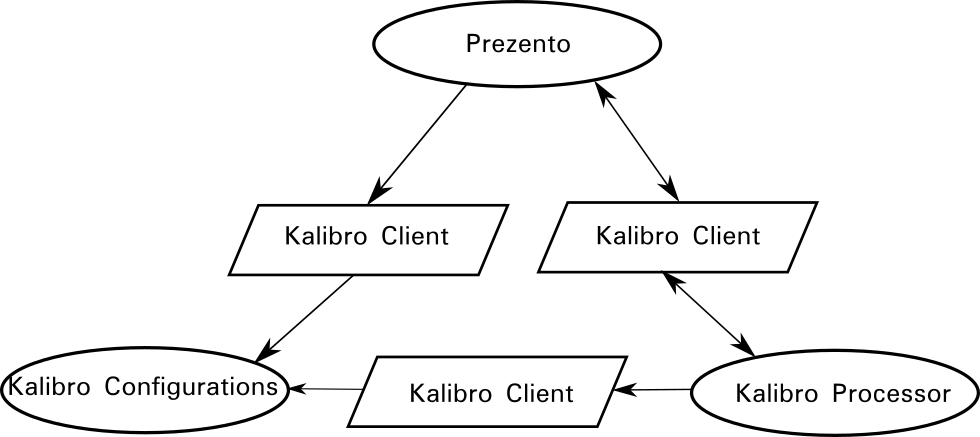
\includegraphics[width=.8\linewidth]{images/mezuro-architecturev3.png}
  \caption{Current Mezuro architecture.}
  \label{fig:architecture-2}
\end{figure}

The current Mezuro state is specified in Figure \ref{fig:architecture-2}.
Ellipses represents softwares involved and parallelograms the communication
interfaces between them. At Mezuro base we have Kalibro, segmented in three
smaller entities: Kalibro Processor, responsible for processing and evaluating
metrics; Kalibro Configurations, responsible for metrics definitions and
configurations; and Kalibro Client, responsible for interoperate communications
between these entities.  Prezento, the presentation layer, mainly communicates
with Kalibro Processor and Kalibro Configurations, via the Kalibro Client
interface.
